\documentclass[]{article}

% Review comments stuff
% -----------------------------------------
\usepackage[english]{babel}
\usepackage[dvipsnames,svgnames,x11names]{xcolor}
\usepackage[markup=underlined]{changes}
% Use "final" option to remove all tracking markups
% \usepackage[final]{changes}

\definechangesauthor[color=BrickRed]{RB}

% Alternative definition to have the remarks
% in the margins instead of footnotes
\usepackage{todonotes}
\setlength{\marginparwidth}{3cm}
\makeatletter
\setremarkmarkup{\todo[color=Changes@Color#1!20,size=\scriptsize]{#1: #2}}
\makeatother

%% Definition of a plain remark/note
\newcommand{\note}[2][]{\added[#1,remark={#2}]{}}

% -----------------------------------------

% Increase text width
\usepackage[left=48pt,right=46pt]{geometry}

% Graphics Stuff
\usepackage{graphicx}
\usepackage{float}
\graphicspath{ {images/} }

% Bibliography stuff
\usepackage[round]{natbib}
% Adds bibliography to toc
\usepackage[nottoc,numbib]{tocbibind} 

% Makes toc, urls, figure links
\usepackage{hyperref}

% Format hyperlinks nicer than default way
\usepackage{xcolor}
\hypersetup{colorlinks,linkcolor={blue!80!black},citecolor={blue!80!black},urlcolor={blue!80!black}}

% Title Page
\title{Backup Management and Orchestration System\\
	Final Year Project}
\author{Rob Shelly\\
	Applied Computing\\
	20068406}

\begin{document}
\maketitle
\thispagestyle{empty}

\newpage
\pagenumbering{roman}
\tableofcontents

\newpage
\pagenumbering{arabic}
\section{Introduction}

\subsection{Problem Statement}
In January 2017 GitLab suffered a data loss incident which was widely reported in media. It began with spammers targeting GitLab.com and culminated in an engineer erroneously deleting 300GB of PostgreSQL data in a production. The lost data included merger requests, users and comments \citep{gitlab1}. The bigger story was to come later however when it was realised that GitLabs backup process had failed silently. The backups did not exist, resulting in a total loss of the data. As it transpired, conflicting major versions of \textit{pg\_dump} (a utility for backing up PostgreSQL databases) in use for the backup procedure and the PostgreSQL database resulted in an error, and the procedure failing \citep{gitlab2}.

The incident was widely reported in the tech industry with the story being picked up by a number of outlets including TechCrunch \citeyearpar{lomas} and The Register \citeyearpar{sharwood}. For many, the focal point of the story was the failed backups. The incident highlighted the need for regular verification of backups. A simple way of performing this verification is to regularly restore data. The method of verification is to perform a restore of the data, which can be a mundane and time consuming task. The aim of this project is to create a solution to the issue. A system which can notify administrators when backups have failed may have prevented the data loss in the GitLab ordeal.

\subsection{Aims \& Objectives}
The overall objective is to create a system to test that uncorrupted backups exist and contain valid, readable data. A system will be created that allows sysadmins to test backups and to schedule the regular testing of backups. Thus, the system will have two main objectives:

\begin{itemize}
	\item Eliminate the mundane and time consuming task of backup testing by automating regular tests;
	\item Catch silent failures of the backup procedure by notifying sysadmins of failed backups.
\end{itemize}

\noindent The system will focus on backups of databases. For scope, design will focus on testing MongoDB data and MySQL data, thereby providing a sample of both relational and non-relational database management systems (DBMS). However, the system should be designed such that it can easily modified to test data from others forms of database management systems. As part of the system, the following should be implemented:

\begin{itemize}
	\item \textbf{Web app:} This will act as a front end for the sysadmins run and schedule tests and view results.
	\item \textbf{Automation Server:} This will be the backend of the system. It will take care of retrieving the backup data before performing some sorts of tests.
	\item \textbf{Container Platform:} This will be utilised by the backend to test the server. For example, when testing the data from a MongoDB database, the backend will spin up a container with MongoDB installed in order to verify the data. 
\end{itemize}
% Word count: 887

\section{Technologies}
\note[id=RB]{I've been thinking about word count as I've been reading through the document, and this is the only section where I think you could make some cuts; particularly, the AWS section might be longer than it needs to be. So I would suggest reducing this section a bit, but don't worry about the rest - you'll be close enough to the word count that it won't be an issue!}
\subsection{Docker}
Docker is a container platform for building and managing applications. This project is interested not in Dockers platform but rather in the Docker images that run on the platform. A container image is a modular piece of software. It encapsulates all the code and tools needed to run the software packaged in the image. The image can then be run in a container on any environment using a container platform or service. Thus, it runs independent of the hardware or operating system. The container also isolates the software from other images and software running within the environment \citep{docker}.

The modularity of software makes Docker images appealing for this project. It will allow testing various data base types (e.g. MongoDB, MySQL) through it's software agnostic feature, by deploying an image with the corresponding DBMS software.

\subsection{Amazon Web Services}
The project will make extensive use of Amazon Web Services (AWS) with most or possibly all of the systems infrastructure deployed on AWS, particularly using EC2 and ECS.

EC2 is Amazon's compute service. It allows easy deployment and management of virtual compute resources within the cloud. The flexibility of operating systems, virtual machines (or instances as they are known in AWS) and size of volume of storage make it ideal for this project \citep{ec2}. It will allow the system to create instances with only the necessary resources required (i.e. memory and storage) to test the restoration of a given backup. This keeps the cost of testing to a minimum in keeping with Aim \ref{ao3}.

ECS is Amazon's container management service. It allows Docker images to be easily deployed to and run on  EC2 instances without the need to install Docker on the instances. ECS takes care of much of the container management issues that would arise when deploying a services if implemented through Docker alone. This includes managing port mappings between container ports and host ports, ensuring all containers are accessible if necessary. There is no added cost for using ECS. i.e. the customer only pays for the EC2 instances \citep{ecs}. 

\label{aws-cli} AWS also features a command line interface for building, modifying and destroying infrastructure across all of it's service, including EC2 and ECS. This provides an programmatic method of creating the resources necessary to perform test restorations. The ability to do so allows for the automation of the infrastructure creation and destruction (after testing). This makes AWS an ideal platform for this project as automation is an objective of the project set out in Aim \ref{ao1}. 


\subsection{Jenkins}
Jenkins is an automated build server used to implement continuous integration (CI) and continuous delivery (CD). Configuration and management of the server can be achieved using both a web interface and an API. Jenkins is also extensible through a library of plugins \citep{jenkins}.
 
Jenkins was chosen as a backend service for this project as it, along with it's library of plugins, presents many useful features which will be beneficial to the implementation of the system:
\begin{itemize}
	\item A built in email notification system which can be used to notify users of silently failed backups. This provided the functionality to implement a satisfactory solution to Aim \ref{ao2};
	\item \label{creds-plugin}A Credentials plugin which provides a means of storing various credentials in various forms (e.g. username/password pairs, SSH keys) along with a standard API for Jenkins and other plugins to access and use these credentials \citep{connolly}. This provides a secure manner for using SSH keys for backups servers as well as encryption keys for sensitive backups. This is a key objective of the project outlined in Aim \ref{ao4}.
	\item The ability to schedule jobs to run at regular intervals will provide the functionality described in Aim \ref{ao1}. This eliminates the need for the development of a scheduling system in order to fulfil the systems requirements. 
	\item The REST API can be used to by a user-friendly web based frontend, allowing users who unfamiliar with Jenkins or AWS to perform test restorations. 
\end{itemize}


\subsection{Node}
The frontend of the system will be designed using Node (also known as Node.js). Node is a JavaScript runtime environment for building network applications. It is light-weight and efficient framework through its event driven, no blocking I/O implementation. 

The default package manager of Node is \textit{npm} (for Node Package manager). It is the worlds largest software registry \citep{npm}. The vast registry of free and open source packages available through make Node an attractive choice for this project. Of particular interest are the multiple Node clients for Jenkins. These are Node wrappers for the Jenkins REST API enabling easy integration of the frontend with the Jenkins backend.

Although any of a number of frameworks could have been used, for example Django, Node was chosen for this project due it's light-weight design and extensibility through \textit{npm}, including the aforementioned Jenkins API wrappers.
 
\subsection{React}
The UI element of the frontend will be built using React, a JavaScript library available through \textit{npm} for building user interfaces. React is developed to work independently of other technologies, meaning it can integrated easily with Node and other \textit{npm} packages without the need for refactoring. React builds UI's as a set of components, each managing and their own state and implementing their own render function. This allows fast and efficient of rendering as data changes as only components that are updated will be re-rendered.


% Word count: 1123

\section{Design}
	\subsection{System Architecture Overview}
		The system will comprise of three main components:
		\begin{itemize}
			\item Management Server
			\item User Interface
			\item Disposable instances/containers
		\end{itemize}
		The system will also use existing ECS instances i.e  where backups are stored. Depending on the user of the system there may be multiple backup servers in different location (such as AWS regions) or for different data types (relational and non-relational databases).
		
		\begin{figure}[H]
			\setlength{\belowcaptionskip}{15pt plus 3pt minus 2pt}
			\caption{Diagram of System Architecture}
			\centering
			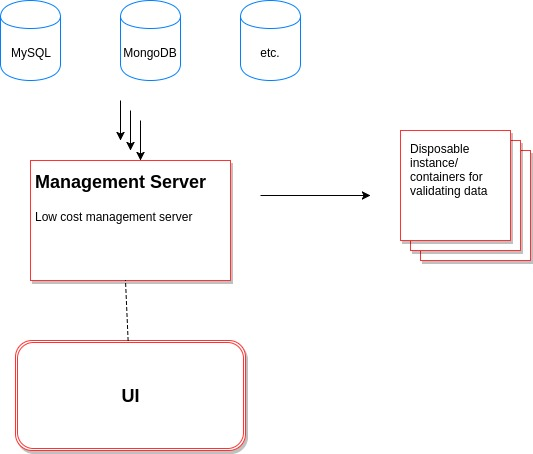
\includegraphics[scale=0.5,keepaspectratio]{diagram}
			\label{fig:diagram}
		\end{figure}
		
		\noindent \textbf{Management Server:} This will be a small low cost AWS instance on which the Jenkins automation server will be installed. The majority of the systems functionality will be carried out and/or orchestrated by this server. Jenkins jobs will copy the backups from their location to a disposable instance and implement the necessary steps to validate them such as importing and and reading.
		
		\noindent \textbf{User Interface:} This will provide a simple user interface (UI) for the system, implemented as a simple web app, hosted on AWS.It will allow users with little knowledge of Jenkins and AWS to perform backup restoration checks by adding a layer of abstraction. Users will be able to run restorations by providing the parameters such as the backup file and it's location. The UI will utilise the Jenkins API to run execute the restoration with the parameters provided.
		
		\noindent\textbf{Disposable Instances:} Disposable infrastructure will be used to perform the restoration. This will consist of EC2 instances running the necessary DBMS to perform the restoration. They can also be destroyed afterwards, destroying the data and therefore maintaining confidentiality.

	\subsection{Formal Modelling}
	\subsubsection{Sequence Diagrams}
		The main function of the systems have been demonstrated below in sequence diagrams. \autoref{fig:seq-run-restore} shows the process of running a single backup restore. This involves a user manually triggering a restoration using the web interface. This triggers a Jenkins job which automates the remaining steps:
		\begin{enumerate}
			\item Backup copied to \textit{restoration} server;
			\item Backup decrypted;
			\item Backup import into DBMS;
			\item Data read from DB;
		\end{enumerate}
		Upon completion the \textit{restoration} server is terminated.

		\autoref{fig:seq-schedule-restore} shows the process of a scheduling regular backup restoration tests. Again, this is triggered by a user from the web interface. The web interface will pass the JSON or XML configuration for a job to the Jenkins server. The server verify the backup server exists before creating the job.
		
		\autoref{fig:seq-delete-restore} Show the process of deleting an existing scheduled job. The user triggers this process from the web interface. This sends a delete commands to the Jenkins server via the API to remove the schedule job. The status of the command, indicating a successful or failed restore, is returned to the user.
		
		\begin{figure}[H]
			\setlength{\belowcaptionskip}{15pt plus 3pt minus 2pt}
			\caption{Run Restore}
			\centering
			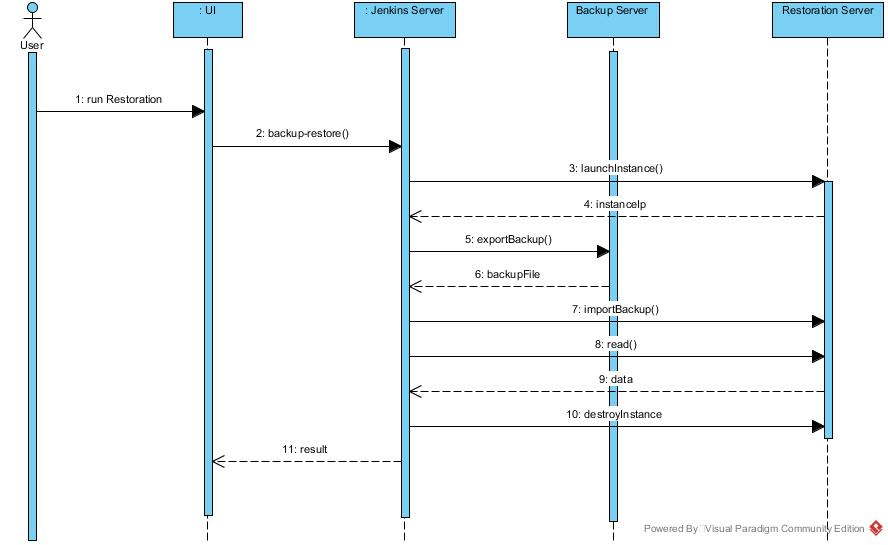
\includegraphics[width=\textwidth,keepaspectratio]{sequence-diagram-run-restore}
			\label{fig:seq-run-restore}
		\end{figure}
		
		\begin{figure}[H]
			\setlength{\belowcaptionskip}{15pt plus 3pt minus 2pt}
			\caption{Schedule Regular Restore}
			\centering
			%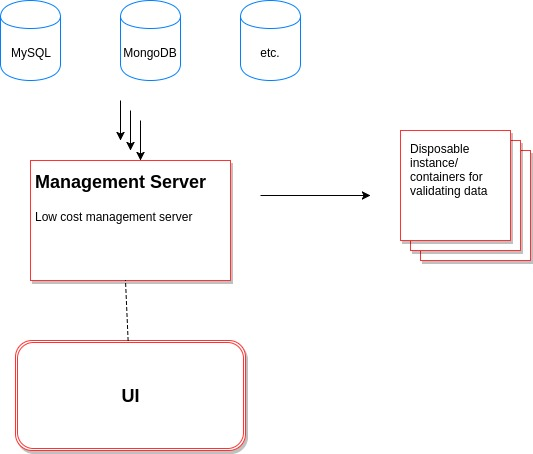
\includegraphics[width=\textwidth,height=\textheight,keepaspectratio]{diagram}
			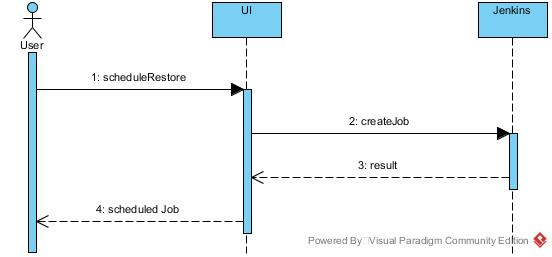
\includegraphics[width=\textwidth,keepaspectratio]{sequence-diagram-schedule-restore}
			\label{fig:seq-schedule-restore}
		\end{figure}
		
		\begin{figure}[H]
			\setlength{\belowcaptionskip}{15pt plus 3pt minus 2pt}
			\caption{Delete Scheduled Restore}
			\centering
			%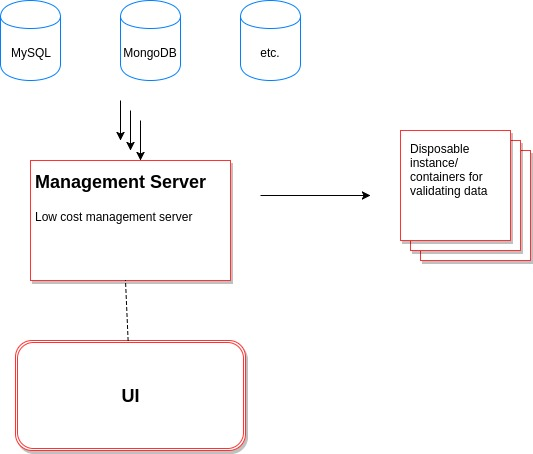
\includegraphics[width=\textwidth,height=\textheight,keepaspectratio]{diagram}
			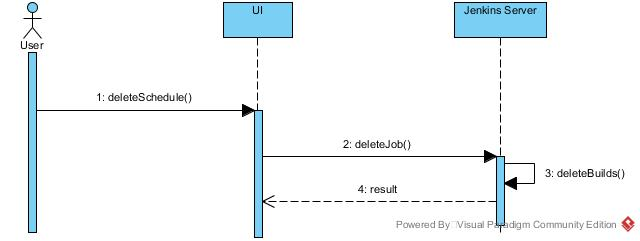
\includegraphics[width=\textwidth,keepaspectratio]{sequence-diagram-delete-schedule}
			\label{fig:seq-delete-restore}
		\end{figure}
	
	\subsubsection{User Stories} \label{user-stories}
   
		User stories are provided in \autoref{table:user-stories}. Two types of system users and their privileges are described below;
		
		\textbf{Managers} control security aspects of the system:
		\begin{itemize}
			\item Add and remove regular users;
			\item Manage SSH keys and decryption keys.
		\end{itemize}
		\textbf{Regular Users} will perform the day-to-day tasks of the system:
		\begin{itemize}
			\item Perform resorations;
			\item Schedule restorations;
			\item View restoration results;
		\end{itemize}
		
		\begin{table}[H]
			\small
			\centering
			\setlength{\belowcaptionskip}{15pt plus 3pt minus 2pt}
			\caption{User Stories}
                         
			\begin{tabular}{|l|l|p{0.39\linewidth}|p{0.39\linewidth}|} \hline
				\textbf{\#} & \textbf{As a} & \textbf{I want to be able to} & \textbf{so that} \\ \hline
				US1 & manager & implement a user system & I control who can run backup restores \\ \hline
				US1.1 & manager & add my team members to the system & they can run backup restores \\ \hline
				US1.2 & manager & remove users from the system & former team members no longer have access \\ \hline
				US2 & manager & add and control sensitive information within the system & I can implement a security policy \\ \hline
				US2.2 & manager & securely store credentials within the system & they don't need to be entered every time a restore is executed \\ \hline
				US2.3 & manager & add SSH keys for backup server & the system has secure access backup server \\ \hline
				US2.4 & manager & add decryption keys for backups & encrypted backups can be decrypted for testing \\ \hline
				US2.5 & manager & delete SSH keys & expired/outdated credentials are no longer stored \\ \hline
				US2.6 & manager & delete decryption keys & expired/outdated credentials are no longer stored \\ \hline
				US3 & manager & execute all same tasks as a regular user & I don't need a second set of credentials to run restores myself \\ \hline
				US4 & user & login & I can run restores \\ \hline
				US5 & user & logout & I avoid potential unauthorised access \\ \hline
				US6 & user & run a test restoration of a backup & I can verify that the backup exists, is a valid file, and is readable \\ \hline
				US6.1 & user & run a test by filling out a simple form with basic parameters (location, filename) of the backup to test & I can easily run a restore of a specific backup without needing to worry about the implementation \\ \hline
				US6.2 & user & view the current status of a running restoration & I can review the progress of long running restores \\ \hline
				US6.3 & user & check if a backup failed or succeeded & I can immediately investigate any failed backups \\ \hline
				US7 & user & create a schedule of automated restores for a given backup & I don't have to manually execute them myself on a regular basis \\ \hline
				US7.1 & user & choose the frequency of automated restores within a schedule, from daily through weekly to monthly & I control how often different backups are tested \\ \hline
				US7.2 & user & check if an automated restoration has started & I can verify my schedule is working correctly \\ \hline
				US7.3 & user & check the results of an automated restore & I can immediately investigate any failed backups \\ \hline
				US7.4 & user & view the all past results of an automated restore schedule & view the consistency of my backups success \\ \hline
				US7.5 & user & modify a scheduled restore & I can change the frequency of a scheduled restore \\ \hline
				US7.6 & user & the parameters of a schedule & any changes to the backups, such as location, will be reflect in the restoration schedule \\ \hline
				US7.7 & user & delete regularly scheduled restores & old backups/deleted backups are no longer tested \\ \hline 

US8 & user & view feedback of a failed restore & I might gain an insight into the fault in the backup \\ \hline
				US9 & user & notified when a restoration fails & silent, unnoticed fails are avoided \\ \hline
			\end{tabular}
			\label{table:user-stories}
		\end{table}
		

        
	\subsection{Front End Design}
	\subsubsection{Wireframes}
	
		Wireframes for the frontend are shown below. 
        
        \autoref{fig:homepage} shows the homepage. It includes the following components:
		\begin{itemize}
			\item Form for running a restore;
			\item Form for creating a restore schedule;
			\item List of schedules (including links).
		\end{itemize}
		\autoref{fig:scheduled} shows the details and past results of a scheduled restore.
		
		
		\begin{figure}[H]
			\setlength{\belowcaptionskip}{15pt plus 3pt minus 2pt}
			\caption{Homepage}
			\centering
			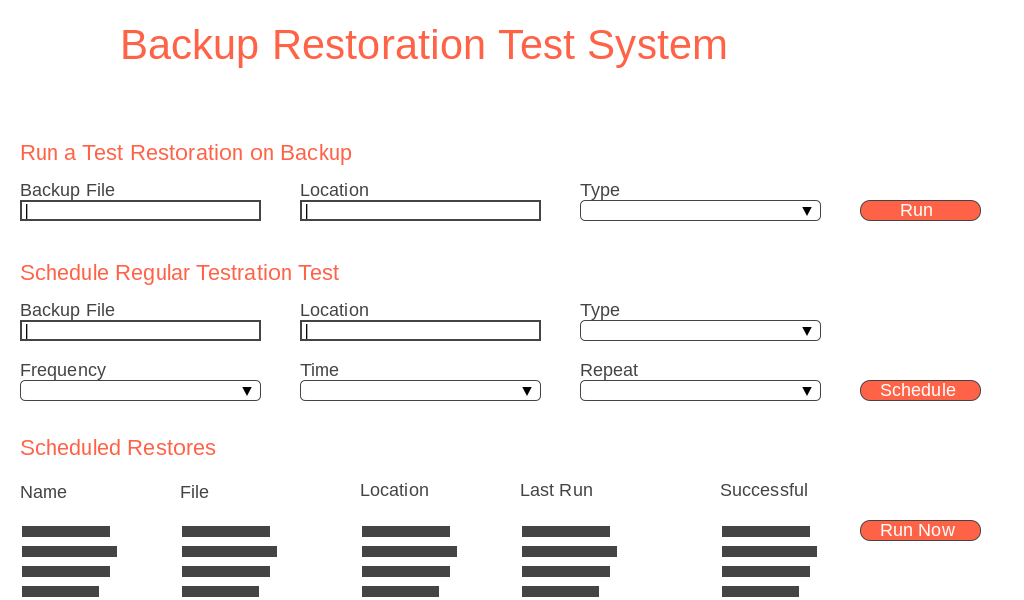
\includegraphics[width=\textwidth,keepaspectratio]{wireframe-homepage}
			\label{fig:homepage}
		\end{figure}
		
		\begin{figure}[H]
			\setlength{\belowcaptionskip}{15pt plus 3pt minus 2pt}
			\caption{Scheduled Restore}
			\centering
			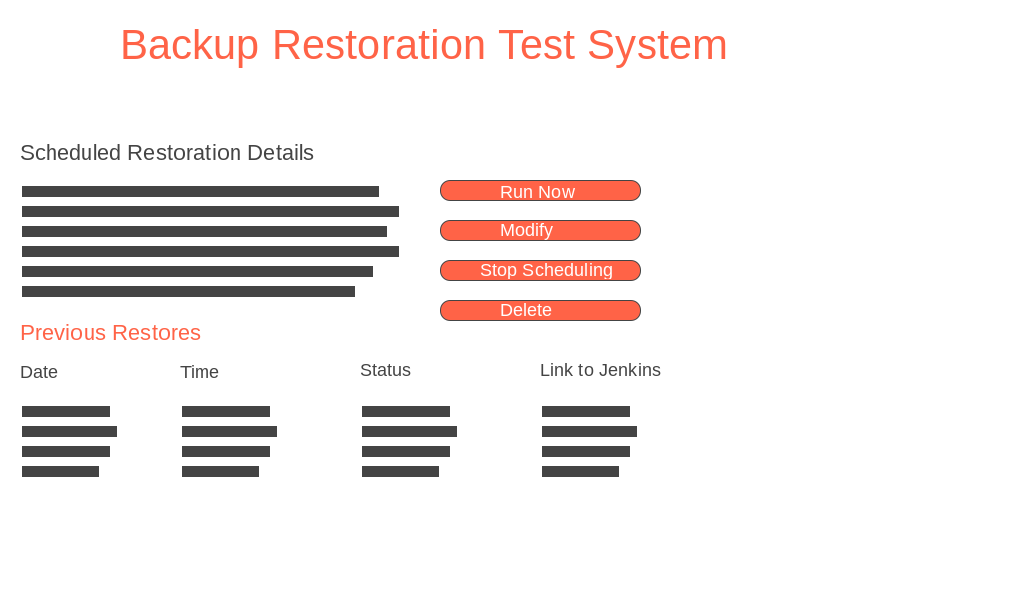
\includegraphics[width=\textwidth,keepaspectratio]{wireframe-scheduled-restore}
			\label{fig:scheduled}
		\end{figure}
	
% Word count: 970

\section{Methodology}
	\subsection{Agile}
	The design methodology chosen for this project is Agile. Agile takes an iterative approach to designing and delivering products. It's a goal driven methodology that aims to build and deliver software incrementally from the beginning of the project, in contrast with traditional approaches such as Waterfall which deliver in one final stage. A notable aspect of Agile is user stories. The project is broken into small sections of functionality which can be independently developed and delivered upon completion \citep{rasmusson}. A number of user stories have been described \hyperref[user-stories]{above}, detailing the main requirements of this project. 
	
	\subsubsection{Scrum}
	
	A particular Agile framework which will be used for this project is Scrum. Scrum defines terms used to organise development:
	\begin{itemize}
		\item \textbf{Product Backlog:} This is a prioritised list of jobs which need to be completed. In its entirety, it represents the full development of the project, i.e. all the work required to deliver the final product.
		\item \textbf{Sprints:} Development is divided into a number of equal length periods (often two or three weeks) of work known as sprints. Each sprint has it's own small goal to achieve, with some items from the head of the product backlog being developed. This project will be organized into six sprints of two weeks each.
		\item \textbf{Daily Scrum:} The daily scrum, also known as daily \textit{standup}, is a daily meeting at which team members meet to discuss progress and address issues encountered.
		\item \textbf{Sprint Reviews:} At the end of each sprint a review of the work completed is carried out. The next sprint will then begin, developing the next group of items from the backlog being\citep{scrum}.
	\end{itemize}
	Also defined are a number of roles:
	\begin{itemize}
		\item \textbf{Product Owner:} The product owner is responsible for the backlog. They are responsible for ensuring the development succeeds in its goals by implementing the work laid out in the backlog. It is the duty of the product owner to prioritise the backlog. 
		\item \textbf{Scrum Master:} The scrum master is responsible for maintaining focus on the current batch of backlog items during each sprint \cite{agile}.
	\end{itemize}
	
	Scrum is an ideal model for developing this project. The Product Owner will be Red Hat and the role of scrum master will be played by the project supervisor. Development will broken into six sprints of two weeks. However, as this is not a team project, daily stand-up meetings will not be held. Rather, meetings with the scrum master on weekly basis and meetings with the product owner on a similar schedule as needed. The user stories which have been used to describe the requirements of the project will be organised into the product backlog.
	
	\subsection{CI/CD with Jenkins}
	Continuous Integration/Continuous Deployment (or continuous Delivery) is a development concept that focuses on the frequent and automated testing building and releasing of code. It aims to remove the large workload required when it is time to release a version or update of a product by performing the same process in a automated manner on every code commit \citep{pittet}.
	
	Continuous integration refers to preparing the code for release as often as code commits are performed. For example, running tests and building Docker images on each commit meaning code is prepared for release at each stage of development, instead of when it come to release time \citep{ramos}.
	Continuous Deployment is a step beyond Continuous Integration. After the code is built it is deployed to a server. However, this may be a development server. Pushing the built code to production requires a manual trigger. Continuous Delivery automates this final manual trigger, meaning the entire process of moving code through testing, building and deployment to production is entirely automated \citep{ellingwood}.
	
	For this project, CI/CD (continuous development in this case) will be implemented using a Jenkins automated build server.Each time a commit of the frontend source code is push to GitHub, the app will be built as a Docker image and deployed to ECS by Jenkins on every code commit. This workflow is shown in \autoref{fig:cicd}.
	
	\begin{figure}[H]
		\setlength{\belowcaptionskip}{15pt plus 3pt minus 2pt}
		\caption{CI/CD of Wep App}
		\centering
		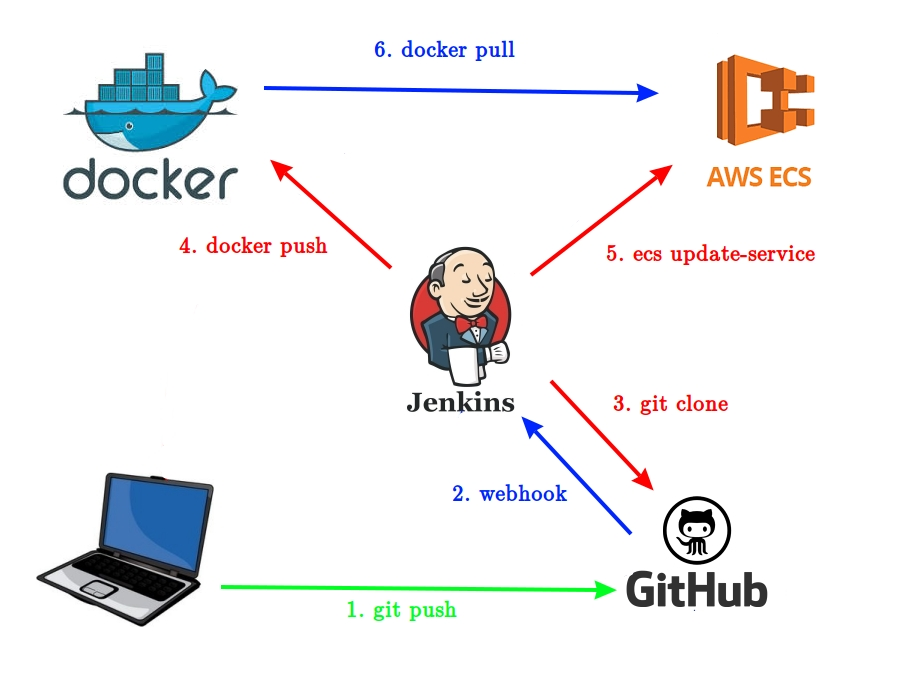
\includegraphics[scale=0.5,keepaspectratio]{cicd}
		\label{fig:cicd}
	\end{figure}
	
	\subsection{Jira}
	In conjunction with the Scrum framework the Jira development tool will be used. Jira is a project management tool which allows the creation and tracking of tasks or issues. The product backlog, comprising of the project user stories, can be created within the management tool with tasks created for each of the stories on the backlog. Each task can then be prioritised as the in the manner chosen by the product owner \citep{jira}.
	
	A number of Jira's feature make it an ideal tool to aid in the organisation of this project:
	\begin{itemize}
		\item \textbf{Issue Tracking:} Progress on issues within the product backlog can be tracked though useful status tags such as In Progress, On Hold and Done. This provides a mechanism for recording progress on each of the user stories which implemented for this project. 
		\item \textbf{Scrum Boards: } Sprints can be represented using Scrum boards. Scrum boards provide a way of organising the issues in a visual manner, grouping them into logical categories (To Do, In Progress, Done) focus on the progress of the current sprint \cite{scruminc}.
	\end{itemize}
	
	\subsection{Completion and Handover}
	Due to the goal driven and iterative aspects of Agile methodology, a clear idea of a completed project is required. This will provide the final goal to work towards and a clear understanding of when this goal is reached. Accordingly, a \textit{Definition of Done} is a a key element of Scrum \citep{panchal}. The design methodology for this project will have the following stipulations:
	
	\noindent The \textit{Definition of Done} for each sprint will be as follows:
	
	\begin{itemize}
		\item Each issue (user story) has been tracked within Jira.
		\item Each issue is implemented;
		\item Each code for each issue has been documented.
		\item A sprint review meeting has been held;		
	\end{itemize}
	
	\noindent The \textit{Definition of Done} for the project  will be as follows:
	
	\begin{itemize}
		\item User stories have been categorised as \textit{Functional Goals} and \textit{Stretch Goals} in an initial backlog refinement;
		\item All \textit{functional} user stories have been implemented with considerations made for \textit{stretch goals};
		\item All code committed to GitHub repository;
		\item All code documented;
		\item Latest image of web app deployed to ECS through CI/CD;
		\item Latest image available on Docker Hub registry;
		\item A working deployment of the entire system is running and available for demonstration.
	\end{itemize}
	 
	 \noindent The following deliverables will be required for completion of the project. 
	 \begin{itemize}
	 	\item Presentation of the project;
	 	\item Project report;
	 	\item Descriptive poster of project;
	 	\item Demonstrative video of project feature.
	 \end{itemize}
\section{Implementation of Prototype}
	\subsection{Sprint 1}
	\subsection{Sprint 2}
	\subsection{Sprint 3}
% Word Count 273

\section{Summary}
	\subsection{Review of Work Completed}
	As part of the research phase of the project a number if initial task have been completed:
	\begin{itemize}
		\item A Jenkins server has been deployed to AWS for use during POCs;
		\item a CI/CD workflow for the frontend was created for fronted which can deploy the frontend to ECS;
		\item A backup validation POC has been completed which demonstrated the feasibility of performing backups restorations and verified the ability to validate the data to the extent that users can be satisfied the backups are working;
		\item A user-rules POC was carried out which verified that users will be able to run restorations via a simple and user-friendly interface, abstracting the implementation of the validation process;
		\item A security POC was to demonstrate that the proposed system can be applied to encrypted backups, decrypting them for validation in a secure manner.
	\end{itemize}
	
	\subsection{Work to Complete}
	The next steps for the project are outline below in the order in which they will be implemented:
	\begin{enumerate}
		\item Integrate each of the three POCs to provide a skeleton system for further development. This will consist of the following tasks:
		\begin{itemize}
			\item Adding the decryption functionality of \hyperref[poc1]{POC3} to the basic restoration job completed in \hyperref[poc1]{POC1};
			\item Hook the frontend to the job created in \hyperref[poc1]{POC1} using the methods demonstrated in \hyperref[poc1]{POC2}.
		\end{itemize}
		\item Hold a product backlog refinement session prior to the commencement of the first sprint in which the user stories are added to the backlog and prioritised;
		\item Commence the first sprint, choosing a number of user stories from the top of the backlog;
		\item Begin working on the user stories as per sprint goals.
	\end{enumerate}



\newpage
\renewcommand*{\bibfont}{\raggedright}
\bibliographystyle{plainnat}
\bibliography{bibliography/bibtex}

\end{document}


